% MBD, Agile and CI/CD as Factors of One Pipeline -- IEEE ISIE 2027 regular paper (6 pages, IEEE two-column).
% Draft v1, 2026-11-11. Every number comes from a script under testbed/ (see the memory files named
% in article-docs/sections/). Bracketed [..] items are placeholders; do not fill them by guessing.
% Build: latexmk -pdf main.tex   (WSL, TeX Live with texlive-publishers)
\documentclass[conference]{IEEEtran}
\usepackage[T1]{fontenc}
\usepackage{amsmath}
\usepackage{graphicx}
\usepackage{booktabs}
\usepackage{array}
\usepackage{multirow}
\usepackage{tikz}
\usetikzlibrary{positioning,arrows.meta,fit,calc}
\usepackage[hidelinks]{hyperref}
\usepackage{orcidlink}

\begin{document}

% Title reworded after the co-author review of 2026-11-14 (point 1): domain first, no leading acronyms.
\title{A Mutation-Based Study of Automotive Embedded Estimator Software: MBD, Agile and CI/CD as Factors of One Pipeline}

% ISIE 2027 paper-submission page (read 2026-11-13): 6 pages "including title, authors, affiliations",
% no anonymisation instruction (t-0036). Authors, order and affiliation given by the first author on
% 2026-11-13 (d-0015): Osvaldo, Max, Rafael, Jeferson. The source block gave no affiliation mark for Rafael.
% Order changed on Overleaf by Max Mauro Dias Santos (2026-11-14 02:44 and again 2026-11-15 00:25 UTC):
% Osvaldo, Rafael, Jeferson, Max. Confirmed by the first author 2026-11-15 (t-0037). Rafael is also UTFPR, so
% all four share one affiliation and the reference marks are dropped (IEEE single-affiliation form).
\author{\IEEEauthorblockN{Osvaldo Janeri Filho\,\orcidlink{0009-0000-5869-4947},
Rafael Santos Dominguez\,\orcidlink{0009-0007-2827-618X},
Jeferson Jos\'e de Lima\,\orcidlink{0000-0001-6342-6162}, and Max Mauro Dias Santos\,\orcidlink{0000-0001-7877-3554}}
\IEEEauthorblockA{Department of Electronics, Federal Technological University of
Paran\'a -- Ponta Grossa\\Ponta Grossa, PR 84.017-220, Brazil}}

\maketitle

\begin{abstract}
Vehicle estimators, such as a battery's state of charge or the fuel used, are verified with model-based
design (MBD), Agile iteration and continuous integration and delivery (CI/CD), practices often compared as
alternatives. We turn them into factors of one pipeline: which
verification stages run (unit tests and model-, software- and processor-in-the-loop testing), the increment
size that Agile practice sets (commits verified together) and the release
trigger. In a battery state-of-charge observer and a fuel-flow virtual sensor we injected 205 defects
(mutants), 102 of which degrade the estimate on recorded laboratory and field data, and ran each on a host
PC, an emulator and a general-purpose Arm Cortex-M4F board. Unit tests caught 38 and 68\,\% of these,
respectively, while executing 97--100\,\% of the lines: their expected
values come from the mutated specification, so they missed every model-level defect. In an exploratory
re-analysis, requirement tests caught all of them on host C code alone, so the gain came from the test suite
more than from the stage, and the board added none. In a replay that assumes defects do
not mask each other, the increment size changed only latency, from under a minute to about 9\,h at an assumed
2\,h commit spacing, and board runs multiplied compute by 6 to 19. With the same compiled binary on both
platforms, a confirmatory experiment on a third subject, a stationary battery-rack estimator, found no functional verdict that only the board produced: the platforms agreed
on 84 of 84 control mutants, and the emulator caught all 26 uninitialised-state mutants, also at two more
optimisation levels and on a second board. For this computation-only code the board was
needed only for timing, where the emulator's instruction count mis-scaled regressions in both directions and
the two boards disagreed.
\end{abstract}

\begin{IEEEkeywords}
automotive software, model-based design, agile development, continuous integration, processor-in-the-loop, mutation testing
\end{IEEEkeywords}

% ---------------------------------------------------------------------------------------------------
\section{Introduction}

Much of the software in a vehicle estimates what no sensor measures: a battery management system computes
the state of charge from current and voltage, and a telematics unit infers the fuel used from airflow and
engine speed read over the diagnostics port. A defect in such an estimator yields a wrong range or consumption figure without any visible
failure, so how the code is verified is a practical question for automotive teams. Three families of practice
are used, often presented side by side. Model-based design (MBD) verifies in stages that come ever closer to
the vehicle and cost ever more to run (Fig.~\ref{fig:pipeline}): the tests first run on a simulation model
before any code exists (model-in-the-loop, MIL), then on the C code compiled for a desktop computer
(software-in-the-loop, SIL), then on the target microcontroller (processor-in-the-loop, PIL), and finally with
the controller connected to a simulated plant (hardware-in-the-loop, HIL). Agile methods deliver small
increments and integrate them often. Continuous integration and delivery (CI/CD) automate the build, the tests
and the release of every change. Industrial pipelines already combine them: software models of electronic
control units (ECUs), called virtual ECUs, run SIL tests inside CI~\cite{kavgic2026,kim2026}, and DevOps practice, which
joins development and operations, is being carried into HIL work~\cite{schlatzer2025}. The comparisons that
guide such choices, however, are often presented as tables of strengths and weaknesses that ask which method
to adopt.

We do not compare the methods as alternatives. We turn each into a factor that can be switched on and off in
one pipeline and measure what each changes. Agile and CI/CD overlap here: Agile asks for working software delivered
frequently, preferring the shorter timescale~\cite{agilemanifesto}, and CI/CD automates the integration of each
increment. MBD contributes the verification stages that run. Agile contributes the increment size, the
number of commits verified together, which CI/CD also exposes. CI/CD's own contribution is the trigger:
automatic on every change, or a gated manual release. Team practices are not studied, so the Agile factor is
narrow by design. With known injected defects, and recorded laboratory and field data as the oracle, i.e.\ the reference that decides whether an estimate is still correct, the effect of each
factor can be measured on the same defects, in paired comparisons.

We ask three questions:
\begin{itemize}
\item \textbf{RQ1} (what is caught): how much does each verification stage, and the test suite it runs,
add to the detection of defects that degrade the estimate on recorded data (field-relevant), and at what cost?
\item \textbf{RQ2} (when it is caught): how do batch size and trigger change feedback latency and
compute?
\item \textbf{RQ3} (where it must run): when does the execution platform (host, emulator, real board)
change a verdict, and what is the cheapest placement of the stages that keeps detection?
\end{itemize}
RQ1's protocol was committed before its run (locally; Section~\ref{sec:threats}); RQ2's replay was designed
after S1's first results. RQ3 was added after the first experiment showed host/emulator/board
disagreements; it was then tested in a separate confirmatory experiment, frozen before it ran, on new
mutants and a new subject. The hypothesis, committed before the first run, that the stages are
non-redundant was partly refuted.

The contributions are: (i) an open pipeline (OpenModelica for model simulation, gcc for host builds, the
QEMU emulator, and a real Cortex-M4 board on the FIT IoT-LAB remote testbed~\cite{adjih2015}) applied to three subjects built from public recorded data; (ii) a paired
measurement of detection per stage and test suite on 205 mutants, and a replay, built from the measured stage
costs and verdicts, of latency and compute per increment size and trigger; (iii) a
confirmatory test showing that, with one binary and for computation-only code without peripherals or
interrupts, an emulator reproduces the board's functional verdicts and the board is needed only for timing; and (iv) a preliminary tiered placement of the stages derived
from (iii) and replayed on functional verdicts only. Scripts, protocols and raw results are available at
\url{https://github.com/ojaneri/mbd-agile-cicd-factors}.

% ---------------------------------------------------------------------------------------------------
\section{Related Work}

Several works build pipelines that join model-based artefacts and CI/CD. M\"ortstrand \emph{et
al.}~\cite{mortstrand2023} add a CI/CD pipeline to a model-based tool for finding designs that meet timing requirements and apply it to two
automotive use cases; Dmitriev \emph{et al.}~\cite{dmitriev2020} derive an automated MBD process from
avionics objectives. Kim \emph{et al.}~\cite{kim2026} build real-ECU and virtual-ECU images in
parallel under Jenkins and check functional equivalence; Schlatzer \emph{et al.}~\cite{schlatzer2025} apply
DevOps to HIL simulation development, leaving a lead-time assessment to future work.

Two works study moving tests between platforms. Kavgic \emph{et al.}~\cite{kavgic2026} run six virtual ECUs
in a SiL setup within CI and assess how many existing HiL tests transfer to SiL; earlier defect detection
is argued, not measured; Fu \emph{et al.}~\cite{fu2022} analyse CI failures in industrial HIL projects. On
cadence, Beheshtian \emph{et al.}~\cite{beheshtian2022} measure batching
and bisection strategies for general software builds, without an embedded target. Injected defects in an MBD setting appear in Manuel \emph{et al.}~\cite{manuel2025}, who
inject sensor faults into a Simulink model with AUTOSAR diagnostic blocks and assess test coverage at the
MIL stage.

In a dated search of IEEE Xplore and Scopus (November 2026) we did not find a paired measurement of defect
detection per stage (MIL, SIL, PIL) combined with integration cadence, with known injected defects, in an
embedded MBD pipeline; nor a test of whether an emulator can replace the target board for a given defect
class. The search was not exhaustive (ACM DL and SAE were not covered).

% ---------------------------------------------------------------------------------------------------
\section{Integrated Pipeline and Experimental Design}

\begin{figure}[t]
\centering
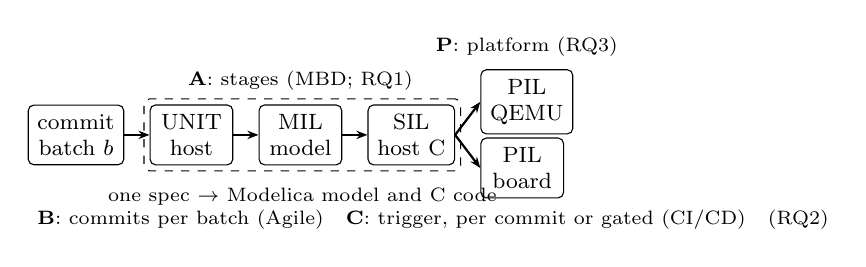
\begin{tikzpicture}[
  st/.style={draw, rounded corners=2pt, minimum width=1.05cm, minimum height=0.62cm, font=\footnotesize, align=center},
  ar/.style={-{Stealth[length=4pt]}, thick},
  lb/.style={font=\scriptsize, align=center},
  node distance=0.32cm]
\node[st] (c) {commit\\ batch $b$};
\node[st, right=of c] (u) {UNIT\\ host};
\node[st, right=of u] (m) {MIL\\ model};
\node[st, right=of m] (s) {SIL\\ host C};
\node[st, right=of s, yshift=0.42cm] (q) {PIL\\ QEMU};
\node[st, right=of s, yshift=-0.42cm] (b) {PIL\\ board};
\draw[ar] (c) -- (u); \draw[ar] (u) -- (m); \draw[ar] (m) -- (s);
\draw[ar] (s.east) -- (q.west); \draw[ar] (s.east) -- (b.west);
\node[lb, above=0.06cm of m] {\textbf{A}: stages (MBD; RQ1)};
\node[lb, above=0.04cm of q] {\textbf{P}: platform (RQ3)};
\node[draw, dashed, rounded corners=2pt, fit=(u)(m)(s), inner sep=2pt] (spec) {};
\node[lb, below=0.08cm of spec] {one spec $\rightarrow$ Modelica model and C code};
\node[lb, anchor=north west] at ($(c.south west)+(0,-0.45)$) {\textbf{B}: commits per batch (Agile)\quad \textbf{C}: trigger, per commit or gated (CI/CD)\quad (RQ2)};
\end{tikzpicture}
\caption{The pipeline and its factors. A selects which stages run: A0 runs only the unit tests, A1 adds
MIL, A2 adds SIL and A3 adds PIL. B is the number of commits verified together; C is the trigger; P is the
platform on which PIL runs. The Modelica model is the estimator itself, without a plant.}
\label{fig:pipeline}
\end{figure}

\subsection{Subjects and field oracles}
\begin{table}[t]
\caption{The three subjects (estimators) and their mutants. OCV: open-circuit voltage; RMSE: root-mean-square
error; the field oracle compares a mutant with the original code on held-out recordings.}
\label{tab:subj}
\centering
\footnotesize
\setlength{\tabcolsep}{2.5pt}
\begin{tabular}{@{}>{\raggedright\arraybackslash}p{0.16\columnwidth}>{\raggedright\arraybackslash}p{0.25\columnwidth}>{\raggedright\arraybackslash}p{0.28\columnwidth}>{\raggedright\arraybackslash}p{0.22\columnwidth}@{}}
\toprule
 & S1 (SoC) & S2 (fuel) & S3 (rack)\\
\midrule
Estimates & battery state of charge & fuel used per tank & stationary battery-rack temperature, derating\\
Model & 1RC circuit, 11-knot OCV table, 1\,s step & airflow-based flow, fuel cut-off, trims, clamped integrator & first-order thermal, derating latch\\
Inputs & current, voltage & airflow, engine speed, throttle, fuel trims & current, reference temp., reset\\
Data & laboratory drive-cycle tests of one LG HG2 cell, 25\,\textdegree C~\cite{lghg2data} & OBD-II log of a 2012 car with refuelling~\cite{obd2data} & storage-system field data~\cite{bessdata}\\
Field oracle fails if & SoC (0--1) RMSE $+0.005$ or max.\ error $+0.02$, any of 4 cycles & volume error $+2$ points, any of 5 tanks & not used\\
Mutants (model, code) & 130 (46, 84) & 75 (23, 52) & 93 (28, 65)\\
Field-relevant & 68 & 34 & --\\
\bottomrule
\end{tabular}
\end{table}
All three subjects are estimators identified on public recorded data (Table~\ref{tab:subj}). S1 computes a
battery's state of charge (SoC) from current and terminal voltage with an equivalent-circuit observer and an
open-circuit-voltage (OCV) table. S2 integrates fuel flow from engine signals read over the on-board
diagnostics port (OBD-II) to estimate the fuel used per tank. S3 estimates the temperature of a rack in a
stationary battery storage system, not a vehicle subsystem, and latches a power derating; it is used only in
the confirmatory experiment. Held-out recorded data serve as the
\emph{field oracle}: a mutant is \emph{field-relevant} if it makes the estimate measurably worse than the
original code, by the root-mean-square error (RMSE) or volume thresholds of Table~\ref{tab:subj}. S3's
thermal model is no more accurate than a naive estimate on held-out months (RMSE 0.458 versus
0.449\,\textdegree C, sensor resolution 1\,\textdegree C), so S3 serves as a test subject, not as a useful
virtual sensor. Requirement tests (7, 4 and 5 requirements) and their thresholds were set by us before any
mutant was generated.

\subsection{Pipeline}
For each subject a script generates both a Modelica model and C code from one specification
(Fig.~\ref{fig:pipeline}). The model is the estimator itself, without a plant; the C code is not generated
from the Modelica model, so translation faults are outside this study. UNIT runs hand-written unit tests of
the C functions on the host (four test groups for S1, three for S2) whose expected values are generated from
the specification. MIL simulates the model in OpenModelica, an open-source Modelica simulator, driven by the
requirement test vectors. SIL compiles the C code for the host, runs the same requirement tests and compares
the outputs back-to-back with MIL. PIL cross-compiles the same code for an Arm Cortex-M4F microcontroller,
runs the requirement tests on it, compares back-to-back with SIL and checks a timing budget of twice the
platform's own baseline maximum cycles per step, a relative budget rather than an absolute deadline. The
real target is an STM32L475VG board on FIT IoT-LAB, flashed and read over serial; the emulator is QEMU. We
call the board stage PIL, not HIL, because no plant is connected. \emph{Tools and settings:} OpenModelica
1.27.2; gcc 15.2 on the host and arm-none-eabi-gcc 14.2.1 for the target, both at the usual optimisation
level \texttt{-O2} unless stated; QEMU 10.2.1; the board at 16\,MHz with zero flash wait states and
CRC-checked serial streams; an AMD Ryzen 5 5500 host under WSL Ubuntu.

\subsection{Defects}
Ground truth comes from mutants: small deliberate changes to the program, each standing for one defect, a
technique that goes back to DeMillo \emph{et al.}~\cite{demillo1978} (survey in~\cite{jia2011}); mutants are
a common proxy for real faults~\cite{just2014}. A script of ours applies each operator at every place where it
fits. Model-level operators change parameters, table knots and thresholds, signs, saturations, delays and
resets in the specification,
from which model and code are regenerated, so they reach both; code-level operators (arithmetic and relational
operator replacement, statement deletion, floating-point perturbation, type width) edit only the generated C
code. All 298 mutants (205 in S1 and S2, 93 in S3) compiled and ran (Table~\ref{tab:subj}). Mutants that
change only timing are reported apart, and in S1 and S2 those that no stage flags are screened for equivalence
(Section~\ref{sec:rq1}).

\subsection{Factors, replay and statistics}
Factor A has four cumulative levels (Fig.~\ref{fig:pipeline}): A0 runs only the unit tests, A1 adds MIL, A2
adds SIL and A3 adds PIL. For RQ1 every mutant runs through every stage, so each level's verdict is known for
every mutant. For RQ2 no recorded commit history was
available, so we replay a synthetic sprint: 10 commits, one every 2\,h, each defective with probability 0.3,
the defect drawn from the mutants with their measured per-stage verdicts and stage costs (medians of
the real runs, including board PIL). A defect's verdict does not depend on the other commits in its batch:
defects are assumed not to mask each other, so the replay cannot show the increment size changing detection;
it measures what it does to latency and compute. Batches of $b\in\{1,5,10\}$ commits are verified together
and a failing batch is bisected, as in batching strategies for CI builds~\cite{beheshtian2022}; the trigger
is automatic or a gated release that adds a fixed delay (8\,h), so the trigger's effect on latency holds by
construction. Each configuration is replayed 2000 times with a fixed seed. RQ1 varies A, RQ2 varies B and C
at A2 and A3, and RQ3 varies P, with the tiered placement combining P and a per-sprint schedule; interactions
between factors are not estimated. Detection rates carry Wilson
95\,\% intervals, which describe this mutant population rather than a sample of real defects; times are summarised by
medians, and effect sizes by Cliff's $\delta$. Protocols, mutation operators and analysis scripts were
committed to version control before each run, except RQ2's replay; analyses decided after seeing data are
labelled exploratory.

% ---------------------------------------------------------------------------------------------------
\section{Results}

\subsection{RQ1: what each stage catches}\label{sec:rq1}

\begin{table}[t]
\caption{Detection of field-relevant mutants per cumulative configuration (PIL on the real board),
with Wilson 95\,\% intervals.}
\label{tab:e1}
\centering
\footnotesize
\setlength{\tabcolsep}{3.5pt}
\begin{tabular}{@{}lcc cc@{}}
\toprule
 & \multicolumn{2}{c}{S1 SoC observer ($n=68$)} & \multicolumn{2}{c}{S2 fuel-flow sensor ($n=34$)}\\
\cmidrule(lr){2-3}\cmidrule(l){4-5}
Config & det. & CI (\%) & det. & CI (\%)\\
\midrule
A0 UNIT & 26 & 28--50 & 23 & 51--81\\
A1 +MIL & 52 & 65--85 & 34 & 90--100\\
A2 +SIL & 68 & 95--100 & 34 & 90--100\\
A3 +PIL & 68 & 95--100 & 34 & 90--100\\
\midrule
\multicolumn{5}{@{}p{0.95\columnwidth}@{}}{Median baseline wall time per run, S1: UNIT 0.29\,s, MIL 2.45\,s, SIL 0.29\,s, board PIL 53.5\,s (S2: 18.5\,s).}\\
\bottomrule
\end{tabular}
\end{table}

\begin{figure}[t]
\centering
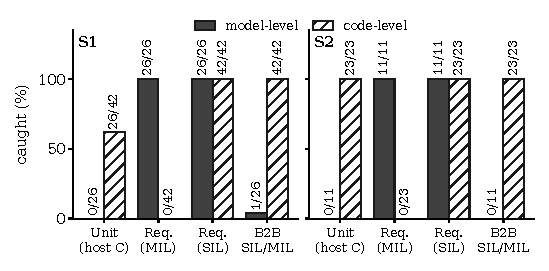
\includegraphics[width=\columnwidth]{figs/fig_suite.pdf}
\caption{Field-relevant mutants caught by each test suite and check, by mutant class (exploratory
re-analysis of the first experiment). Unit: hand-written unit tests on host C; Req.: requirement tests on
the model (MIL) or on host C (SIL); B2B: back-to-back comparison of SIL with MIL. Left S1, right S2;
labels give caught/total.}
\label{fig:suite}
\end{figure}

Table~\ref{tab:e1} gives the detection of field-relevant mutants. Unit tests alone caught 38\,\% (S1) and
68\,\% (S2). MIL raised detection in both subjects, because it is the first stage whose oracle sees
model-level mutants; in S1, SIL added the 16 code-level mutants that unit tests missed. From A2 on, all
field-relevant mutants were detected, and PIL added no field-relevant detection. Because
a 100\,\% rate invites suspicion, we audited it: every field-relevant code mutant in S1 failed a
requirement test at SIL, not only the back-to-back comparison, so the rate is not an artefact of comparing
the code with itself. By construction, MIL cannot see code-level mutants; the back-to-back check saw one
model-level mutant (S1, a numerical divergence above its $10^{-5}$ tolerance).

The hypothesis, committed before the run, that each stage detects some defect class missed by the earlier
ones holds only in part, and factor A changes the test suite together with the stage. An exploratory split by suite
(Fig.~\ref{fig:suite}) shows where the gain comes from. On the same host C code, the requirement tests caught all 68 (S1) and 34
(S2) field-relevant mutants and the unit tests caught 26 and 23, although they executed 97 and 100\,\% of
the lines (83 and 100\,\% of the branches, gcov). The unit tests caught no model-level mutant, because
their expected values come from the mutated specification, and caught 26 of 42 (S1) and 23 of 23 (S2)
code-level ones. Of the 42 field-relevant S1 mutants the unit tests missed, 26 are model-level and 16
code-level, so the gap between the two suites is mostly oracle independence, not coverage (all of it in S2).
MIL, running the requirement tests on the model, caught every
model-level mutant, at about nine times SIL's median cost (8.6 in S1, 9.0 in S2). The detection gain therefore
belongs to the requirement tests, which can run at any level; MIL adds feedback before code exists. PIL was
the only stage that flagged timing regressions (5 mutants in S1, 6 in
S2), as no other stage measures cycles; these did not change the functional field result. A post-run
screening of the mutants no stage flagged on QEMU found 18 of 41 (S1) and 11 of 15 (S2) bit-identical to the
baseline on the host build (one, an initialisation deletion, fails on the board); the other 27 stayed within
the oracles, and on a seeded stress set 7 of them would break a requirement, so the requirement tests are not
exhaustive.

\emph{The platform.} QEMU and the board agreed on 202 of 205 PIL verdicts (Wilson 95.8--99.5\,\%). All three
disagreements, in both directions, were deletions of an initialisation (3 of 6 such mutants, against 0 of 199
others; Fisher exact $p=1.4\times10^{-5}$, post hoc), and the QEMU harness (mps2-an386, semihosting)
differed from the board's, so platform and harness were confounded. This motivated RQ3.

\subsection{RQ2: when defects are caught}

\begin{table}[t]
\caption{Synthetic-sprint replay, automatic trigger: median feedback latency and compute per sprint of 10
commits (2000 replays); other batch sizes are in the artefact.}
\label{tab:e2}
\centering
\footnotesize
\setlength{\tabcolsep}{4pt}
\begin{tabular}{@{}llcccc@{}}
\toprule
 & & \multicolumn{2}{c}{S1} & \multicolumn{2}{c}{S2}\\
\cmidrule(lr){3-4}\cmidrule(l){5-6}
Config & batch & latency & compute & latency & compute\\
\midrule
A2 & 1  & 3\,s   & 36\,s  & 4\,s   & 44\,s\\
A3 & 1  & 57\,s  & 678\,s & 22\,s  & 266\,s\\
A3 & 10 & 9.0\,h & 565\,s & 9.3\,h & 222\,s\\
\bottomrule
\end{tabular}
\end{table}

Table~\ref{tab:e2} shows the replay. With one commit per run and an automatic trigger, a defect was
reported within a minute; with ten commits per run, after about 9\,h, because the defect waits for the batch
to close. A gated manual release added its delay to every cell. Batch size moved latency from seconds to hours
while it changed compute little, since a failing batch is re-run during bisection (Cliff's $\delta$ for
compute, A3 batch 1 against 10: $+0.32$ in S1, $+0.16$ in S2). As the no-masking assumption implies, batching did
not change what was detected: from A2 on, no defect escaped in any replay; at A1, S1 let at least one defect
through in 642 of 2000 sprints, and at A0 the median S1 sprint let one through.
The stage cost mattered only through the board: adding board PIL to every commit multiplied compute per
sprint by 18.7 in S1 and 6.1 in S2 and bought no functional detection. The latency values follow largely
from the assumed commit spacing and gate delay, so the 9\,h figure is a model output. A sensitivity sweep
added after the run (spacing 0.5--8\,h, defect probability 0.1--0.5) left the conclusions unchanged:
ten-commit latency scaled with the spacing, and board PIL multiplied compute by 18.7--20.6 in S1 and 6.1 in S2.

\subsection{RQ3: where a stage must run (confirmatory)}

The confirmatory experiment was frozen before it ran. It uses \emph{one ELF} for QEMU (machine
b-l475e-iot01a) and the board, removing the harness confound. Targets run the test vectors five times: once
as loaded, then four times with the stack below \texttt{main} painted with a different bit pattern; the board
run is made twice, each after a reset. Host arms are SIL, SIL with the state structure overwritten by the same four
patterns, Valgrind memcheck~\cite{nethercote2007} (primary) and MemorySanitizer~\cite{stepanov2015}
(clang 21, secondary). The new mutants are deletions inside the \texttt{init} functions and deleted
initialisations of locals (28 across the three subjects, 26 observable by some arm, 19 of them unseen, i.e.\
not in the first experiment), and timing ladders that add single-cycle (ALU) or 14-cycle (divide)
instructions to the step, enough of them to add 0.25 to 3.0 times the board's baseline cycles. The control set is
S3's first-experiment mutants minus the initialisation deletions and those duplicating a new mutant (84 of 93). The hypotheses were: H1, QEMU and board agree on the control set (Wilson lower
bound $\geq 0.95$); H2, every uninitialised-state mutant the board catches is caught by QEMU (zero
counterexamples); H3, Valgrind catches every such mutant any target catches, at lower median cost than
QEMU; H4, QEMU and board flag the same ALU ladder levels and different divide levels.

\begin{table}[t]
\caption{Uninitialised-state mutants caught per arm (test configuration), of 26 observable and of 19 unseen,
with median wall time per mutant. Wilson 95\,\% intervals.}
\label{tab:e5}
\centering
\footnotesize
\setlength{\tabcolsep}{3.5pt}
\begin{tabular}{@{}lcccr@{}}
\toprule
Arm & caught & CI (\%) & unseen & time\\
\midrule
Host SIL & 22 & 66--94 & 18 & 0.29\,s\\
Host SIL, state overwritten & 25 & 81--99 & 18 & 1.12\,s\\
Host Valgrind (primary) & 25 & 81--99 & 18 & 3.13\,s\\
Host MemorySanitizer (secondary) & 26 & 87--100 & 19 & 0.34\,s\\
QEMU, same ELF, 5 passes & 26 & 87--100 & 19 & 1.91\,s\\
Board, 5 passes $\times$ 2 resets & 26 & 87--100 & 19 & 135\,s\\
\bottomrule
\end{tabular}
\end{table}

All 552 records were valid. \textbf{H1 was supported}: QEMU and the board agreed on 84 of 84 control
mutants (Wilson 95.6--100\,\%). \textbf{H2 was supported}: no uninitialised-state mutant was caught by the
board and missed by QEMU, nor the reverse (Table~\ref{tab:e5}). Without painting, both platforms caught 25 of
26; the painted passes added the last one on both. With the same binary, the disagreement of the first
experiment did not reappear, so it came from the harness and memory layout, not from a property of the
board. \textbf{H3 was not supported} for Valgrind: it missed one mutant (a local left uninitialised in the
OCV inverse of S1) and cost more than QEMU. At \texttt{-O2} the compiler kept that local in a register
holding a defined zero, the original initial value, and memcheck tracks values, not variables; at
\texttt{-O0} and \texttt{-O1} it reported the read, and \texttt{gcc -Wall} warned. MemorySanitizer, the
secondary arm, caught all 26 at 0.34\,s per mutant, about 400 times faster than the board run. Our
prediction that overwriting the state on the host would catch \texttt{init} deletions but not deleted
local initialisations was also wrong: it caught 16 of 17 of the latter, because their garbage values
already fail the requirement tests (plain SIL caught 22 of 26).

\begin{figure}[t]
\centering
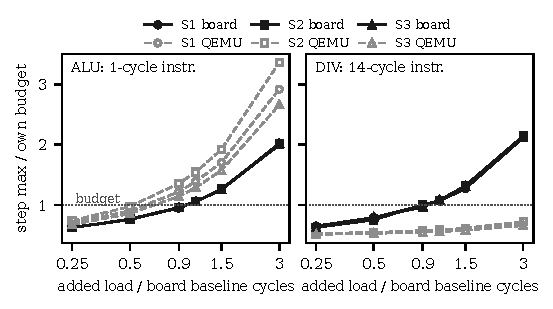
\includegraphics[width=\columnwidth]{figs/fig_h4.pdf}
\caption{Timing ladders: maximum step time of each mutant divided by the platform's own budget (twice its
baseline); above 1 the timing oracle fails. Left, ALU ladder; right, divide ladder; solid lines board,
dashed QEMU. Board values are cycles, QEMU values are ticks under
\texttt{-icount}, an instruction count.}
\label{fig:h4}
\end{figure}

\textbf{H4 was partly supported.} For the divide ladder the platforms differed as predicted: the board
flagged the levels that add 1.1, 1.5 and 3.0 times the baseline cycles, and in S2 also at 0.9, and QEMU flagged none, because
divisions cost about 14 cycles each but count as one instruction (in S3, the 3.0 level added about 420 cycles
but only 30 ticks). For the ALU ladder, against the prediction,
QEMU flagged one level more than the board (0.9 times) in all three subjects. A post-hoc explanation is that
the budget is twice each platform's own baseline and the baseline step runs at about 1.6 cycles per
instruction (107 cycles, 68 instructions in S1), so single-cycle instructions weigh more in an instruction
count than in cycles. An instruction-counting emulator thus mis-scales timing in both directions whenever a
regression's cycles per instruction differ from the baseline's. Fig.~\ref{fig:h4} shows both effects: at the 0.9 ALU level S1
reached 0.95 of its budget on the board and 1.22 on QEMU, while at the 3.0 divide level it reached 2.12 on
the board and 0.69 on QEMU.

\textbf{Tiered placement.} We replayed S3's control set under four placements, with S3's measured stage
costs (UNIT 0.29\,s, MIL 2.49\,s, SIL 0.28\,s, QEMU PIL 0.86\,s, board PIL 30.0\,s per run): A2 (no PIL), A3q
(QEMU PIL per commit), A3b (board PIL per commit) and AT (host and QEMU per commit, board once per sprint).
No control mutant was caught by the board alone, so all four placements had zero escapes. Compute per sprint
was 36.7\,s for A2, 47.1\,s for A3q, 77.1\,s for AT and 396.7\,s for A3b (Cliff's $\delta$ AT against A3b
$-1.0$); latency was 4\,s for AT and A3q and 33\,s for A3b. The per-sprint board run is there for the
multi-cycle timing class of H4, which the control pool did not contain, so the placement was not tested on
the class it exists for.

\textbf{Robustness (addendum).} An addendum, designed after these results and pushed to an external
repository before it ran, counts as a replication outside the confirmatory set. At \texttt{-O0} and
\texttt{-Os}, again with one ELF per level, no uninitialised-state mutant separated board and QEMU; Valgrind
caught all 26 at \texttt{-O0} but missed the same mutant at \texttt{-Os}, and MemorySanitizer caught all 26
at both. A second board, an nRF52840-DK (Cortex-M4F at 64\,MHz, flash cache off), agreed with the
emulator on 84 of 84 control mutants (Wilson 95.6--100\,\%) and caught the same 26 of 28 uninitialised-state
mutants, but with a slower baseline step (158--208 against 107--131 cycles) it flagged fewer timing levels on
4 of 6 ladders (S3 divide: only 3.0 against 1.1--3.0). Functional verdicts thus held across optimisation
levels and boards; timing verdicts differed even between two Cortex-M4F boards.

% ---------------------------------------------------------------------------------------------------
\section{Discussion}

\emph{The factors} acted on different axes: the requirement tests decided what was caught and MIL moved that
verdict before code existed (Table~\ref{tab:e1}); increment size and trigger changed only when
(Table~\ref{tab:e2}); the board mattered for timing (Fig.~\ref{fig:h4}), not function (Table~\ref{tab:e5}).

\emph{Practical placement.} For estimator code of this kind on a Cortex-M4F target, the data support running
UNIT, SIL with a memory sanitiser, and emulated PIL on the same ELF on every commit for functional verdicts,
and keeping the board for a scheduled timing run; MIL remains useful for feedback before code exists. The
timing run has to use the production microcontroller and
memory configuration, since our two Cortex-M4F boards disagreed on which regressions exceeded their
relative budgets. Emulated PIL stays per commit although MemorySanitizer caught the same 26 mutants, because
it runs the cross-compiled target binary, which no host tool checks (no defect specific to it was injected). Two caveats limit this advice: an emulator that counts
instructions is not a timing oracle in either direction, and a sanitiser's result depends on the tool, as the
Valgrind miss shows. Under ISO~26262, using an emulator's verdicts as safety evidence would further require
confidence in it as a software tool~\cite{iso26262p8}; our results support its use for development feedback.

\subsection{Threats to validity}\label{sec:threats}
\emph{Construct.} Mutants stand in for real defects~\cite{just2014}; we report per class and keep timing-only
mutants apart. Model and code come from one specification, so translation and code-generator faults are
absent, and one team wrote the operators, tests and oracles. Agile is reduced to increment size; ceremonies,
team size and collaboration are not measured. The field oracles are relative degradations against recorded data, and the requirement thresholds
are our own. In S2 the field oracle runs on the emulator build, so an initialisation defect that produced a
large error only on the board counted as not field-relevant; field relevance of this class depends on the
platform.
\emph{Internal.} RQ3 was added after seeing the first experiment; its confirmation used new mutants and a new
subject, but S1 and S2 contributed some mutant lines already seen. Detections of 100\,\% were audited. The
increment-size and trigger results come from a synthetic commit stream, not a recorded history; the latency values depend on
the assumed spacing and delay, and the replay assumes defects do not mask each other. The replay replaced the
scripted-backlog design in RQ2's protocol and was designed after S1's first results. Mutants cluster by line
and operator, so they are not independent samples and the Wilson intervals are optimistic. The run scripts were changed once after the confirmatory freeze (build
directories); the affected records were checked valid. The commits that froze the
first experiments and the confirmatory experiment are in a local repository whose external copy dates from
after the runs; the robustness addendum was pushed before it ran. Two incidents during the addendum (a
runner crash and a repeated board calibration) are reported in the artefact.
\emph{External.} Two general-purpose Cortex-M4F boards (STM32L4 at 16\,MHz, zero wait states, flash caches
at reset default; nRF52840 at 64\,MHz, flash cache off), one
emulator, one cross-compiler at three optimisation levels, and three subjects of one
kind (energy and powertrain estimators); S3 is stationary and S1's data are laboratory cell tests. Initial RAM contents depend on the board and its power history; we
report two resets and two boards but cannot bound this. The board's compute multiplier includes this
testbed's flashing and serial I/O. Results may differ for code with deep call trees, interrupts or
caches, and for perception software.

% ---------------------------------------------------------------------------------------------------
\section{Conclusion}

We turned MBD stages, the increment size and the CI/CD trigger into factors of one pipeline and measured
them on 205 injected defects in two automotive estimators, with a confirmatory platform test on a stationary
battery-rack estimator.
Unit tests with near-complete line coverage missed every model-level defect; in an exploratory split,
requirement tests on host C code caught all field-relevant ones. Under the no-masking assumption, the
increment size changed only latency. With the same binary, an emulator reproduced the board's functional
verdicts on this computation-only code, so the board was needed only for timing, where two boards disagreed. A tiered placement used about a fifth
of the compute of a board run on every commit, but was not tested on the timing class it exists for. Future
work: a recorded history with multi-defect batches, timing regressions in the tiered replay, another
compiler, cached cores, and ISO~26262 evidence.

% AI-use disclosure per the IEEE submission policy (author center, read 2026-11-13). Wording given by the
% first author on 2026-11-14 (d-0016; replaces the 2026-11-13 wording, VR4-E-01).
\section*{Acknowledgment}
The authors thank the Federal Technological University of Paran\'a -- Ponta Grossa campus (UTFPR-PG) for its
support. Claude (Anthropic), used under the authors' direction, drafted the text from the authors' results
and notes, helped to write and run the simulation and analysis code that produces the results, and was used
for language editing. The authors reviewed and edited all content and take full responsibility for it.

\bibliographystyle{IEEEtran}
\bibliography{refs}

\end{document}
